\documentclass{article}

% packages
\usepackage{fancyhdr}
\usepackage{geometry}
\usepackage{amsmath}
\usepackage{geometry}
\usepackage{glossaries}
\usepackage{hyperref}
\usepackage{tikz}
\usepackage{multicol}
\usepackage{caption}
\usepackage{background}
\usepackage{wrapfig}

% configurations
\usetikzlibrary{arrows,positioning,shapes.geometric}
\geometry{top=20mm,bottom=30mm,right=20mm,left=20mm}
\makenoidxglossaries
\usepackage{pages/glossary} %importing glossary


% title
\title{\underline{A treatise on Felis Catus, a.k.a \emph{the domestic Cat}}}
\author{Aayush Bajaj}

\backgroundsetup{placement = top, hshift=11cm, vshift=-11cm, scale = 0.4, contents ={\ifnum\value{page}=1 \includegraphics[width=0.5\textwidth]{img/title-cat.png}\else \fi}}
% document
\begin{document}
\maketitle{}

\pagestyle{fancy}
\dotfill

% headerstuff
\section*{Classification}
The dog was the first species to be domesticated $\sim$23,000 years ago (Leonard et al. 2002), and the cat has been one of the last (Larson et al. 2014). The domestic cat is now classified as its own species, the \emph{Felis Catus}. Taxonomically it lies in the \emph{Felidae} family under the \emph{Mammalia} class.\\

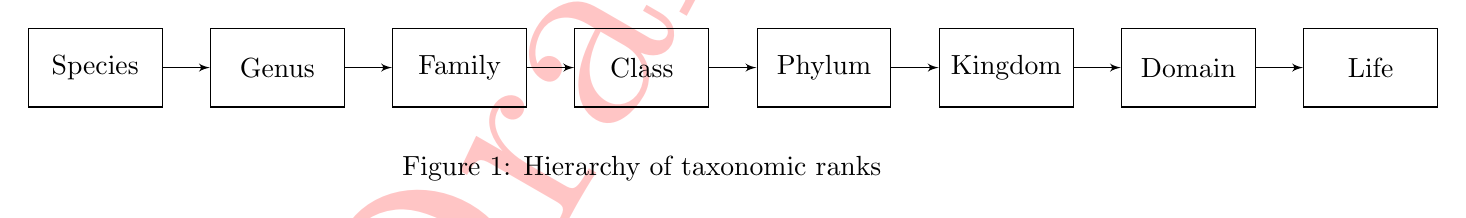
\begin{tikzpicture}[>=latex']
\centering
    \tikzset{block/.style= {draw, rectangle, align=center,minimum width=1.7cm,minimum height=1cm}}
    \node [block] (species) {Species};
    \node [block, right =0.6cm of species] (genus) {Genus};
    \node [block, right =0.6cm of genus] (family) {Family};
    \node [block, right =0.6cm of family] (class) {Class};
    \node [block, right =0.6cm of class] (phylum) {Phylum};
    \node [block, right =0.6cm of phylum] (kingdom) {Kingdom};
    \node [block, right =0.6cm of kingdom] (domain) {Domain};
    \node [block, right =0.6cm of domain] (life) {Life};

    \path[draw,->] (species) edge (genus)
                (genus) edge (family)
                (family) edge (class)
                (class) edge (phylum)
                (phylum) edge (kingdom)
                (kingdom) edge (domain)
                (domain) edge (life)
                ;
    \node [below=1cm, align=flush center,text width=8cm] at (class) { Figure 1: Hierarchy of taxonomic ranks };
\end{tikzpicture}

\section*{Origins}
Originally, the \emph{Felidae} family emerged in Asia during the Miocene period about 11.5 million years ago, but their relationship with \emph{Homo Sapiens} only began 15,000 years ago during the agricultural revolution. Whilst wheat domesticated us, it also enabled us to domesticate the cat. Grain stores and plant crops would attract vermin, which in turn would turn the heads of feral cats. Over the years, the cat became valued as a killer of rodents and thus the symbiotic relationship between man and cat was born. 

\begin{flushright}
\begin{minipage}{8cm}
    \begin{flushleft}
        \emph{It's better to feed one cat than many mice.}
    \end{flushleft}
    \begin{flushright}--- Norwegian proverb\end{flushright}
\end{minipage}
\end{flushright}

\subsection*{Domestication}

\begin{wrapfigure}{R}{0.20\textwidth}
    \centering
    \includegraphics[width=0.20\textwidth]{img/apep-cat.png}
    \caption{The Sun God \emph{Ra} as a cat slaying the demon snake-god \emph{Apep}}
\end{wrapfigure}

Zoologically, this utilisation of cats as crop mercernaries does not constitute \emph{domestication}. Instead this would be accomplished later by the Egyptians who would take control of \textbf{breeding}.\\

Fast forward about 9,000 years now to Mesopotomia in the Fertile Crescent; agriculture is booming, and thus so is the population of African Wildcats. The Egyptians across the Red Sea have their own African Wildcats but want more. Trade routes between the two civilisations are already established and so begins the first social promotion of the \gls{feline}s.\\

The Egyptians kept cats not only as pets, but also believed they were divine creatures of religious significance.\\

Then, as if this deification was not enough, cats attain their second social promotion through political affiliation with \emph{TODO} and cats have become imbued within the culture and society of Ancient Egypt.

\newpage
\subsection*{Spread}

The story continues from Egypt to the rest of the world, where Phoenician Traders begin to smuggle out cats North over the Mediterranean. Due to the strict regulations against this, exportation takes many years, but eventually the cats make it to Greece and Rome and by 500AD the rest of Europe too.\\

Across history, cats have inched forward as deuteragonists; they spread to Northern Europe during the Viking pillages of the \(8^{\text{th}} - 11^{\text{th}}\) centuries, then once they made it to India they traipsed across the Silk Road to the rest of Asia. From there it was easy to prove their usefulness to us on boats as \emph{Health Officials} and convince us to bring them with us on voyages. Traders took them to the Americas, and colonists brought them everywhere else. Ultimately, this spread culminated in the 1788 voyage of the First Fleet to Australia, where Matthew Flinder's brought with him his cat \emph{Trim}.\\

\begin{wrapfigure}{l}{0.25\textwidth}
    \includegraphics[width=0.25\textwidth]{img/crescent.png}
    \caption{The Fertile Crescent}
\end{wrapfigure}


However, the status of cats within society has not always been so elevated. In the 12th and 13th centuries, cats found their way into the folds of pagan religions and were demonised as \emph{evil} creatures. Later, the reign of Christianity and the medieval church saw the persecution of cats and their advertisement as being associated with the devil, necromancers and witches. During this period, cats were tortured and killed, set alight in streets, boiled in water and thrown from heights.\\

Eventually though, the hysteria of the medieval church subsided and cats resumed regaining popularity. The French helped with their positive public sentiment towards cats, and so did the contemporary art. Here is a piece of a Chaucer along with my \emph{favourite} painting by Picasso.\\

\begin{center}\rule{0.5\textwidth}{0.1mm}\end{center}

\begin{multicols}{2}
    \begin{minipage}{0.5\textwidth}
        \begin{flushleft}
            \emph{Lat take a cat, and fostre hym wel with milk,\\
        And tendre flessh, and make his couche of silk,\\
        And lat hym seen a mous go by the wal,\\
        Anon he weyveth milk and flessh and al,\\
        And every deyntee that is in that hous,\\
        Swich appetit he hath to ete a mous.
        }
        \end{flushleft}
        \begin{flushright}--- \emph{The Manciple's Tale}, Geoffrey Chaucer\end{flushright}
    \end{minipage}
    \begin{minipage}{0.5\textwidth}
        \centering
        \includegraphics[width=0.5\textwidth]{img/picasso-cat.png}
        \captionof{figure}{\emph{Cat catching a bird}}
    \end{minipage}
\end{multicols}

\dotfill

\section*{Physiology}
\begin{flushright}
\begin{minipage}{8cm}
    \begin{flushleft}
        \emph{The cat...has a girl's nose, a hare's head,\\
            A tail of snake's venom, claws of a viper,\\
            Feet of cloudberries,\\
            The rest of its body is of the wolf's race.}
    \end{flushleft}
    \begin{flushright}--- Finnish Kalevala (L\"onnrot 1835)\end{flushright}
\end{minipage}
\end{flushright}

\noindent{}The \emph{Felis Catus} is a hunter, she is a direct descendent from the African Wildcats trafficked by the Egyptians above and has the same assets in a more concise form. Born at $\sim$100 grams, the female cat grows to ~3 kg whilst the male grows to ~4kg (\(\pm0.5kg\)). Lengthwise, these animals reach 50 - 60cm, excluding tail-length.\\

These \gls{felid}s are predators. They prefer to kill animals smaller than themselves and as such have acquired a specialised set of tools to hunt these prey. Starting at the foreclaws, these curled and retractable weapons are the primary offensive tool for a cat. They keep these sharp by abrading the outer sheath on trees, scratching posts and furniture. Conversely, the back claws are not curled, less sharp and more knife-like. These claws lack the retraction of the foreclaws and so become dulled with each step.\\

\begin{wrapfigure}{L}{0.35\textwidth}
    \includegraphics[width=0.35\textwidth]{img/cat-skull.png}
    \caption{\emph{Felis Catus} skull}
\end{wrapfigure}
Next we have the teeth, of which there are 30. 12 less than a dog, and 2 less than a human. The reason for this is that their skulls are rather small and so cannot fit a large number of teeth. This however is a double-edged sword as it is this very structure that enables the \emph{Felidae} to deliver the greatest force to size ratio of any other carnivore. Additionally, their jaw joint is different to ours - positioned slightly higher such that their teeth do not close simultaneously, but instead imitate a scissoring motion. The teeth themselves are all pointed; thus what makes them so deadly to mice makes broccoli dangerous to them.\\

The principal sense organs of the cat is their \textbf{eyes}. They possess fantastic visual acuity, with binocular vision for the first \(120^\circ\) and \(80^\circ\) of monocular vision for each eye after that. This leaves them with an \(80^\circ\) blindspot. Nonetheless, this is made up for by their capacity to `see in the dark'. Empirical studies have quantified this sensitivity to light as being 6 times more receptive than a human's eye\(^\dagger\). Contrary to popular belief, cats \emph{can} see colour, though they do lack the physical hardware to see red properly.\\

Finally we have the ears which are controlled by 20 distinct muscles, and are the culprits of the ear-twitching owners notice. Functionally the cats ears are finely tuned, being receptive to frequencies from 200Hz to 100kHz. Humans cannot hear beyond 20kHz, and mice communicate from 20kHz-50kHz. 

\section*{Behaviour}
Cat behaviour can at times be unusual, but majorly these are creatures of regularity. A principal influencer of behaviour is \emph{Father Time}, with whom cats are friendly acquaintances. So much so, that beyond learning their daily feed times they can also distinguish between weekdays and weekends. They can also do a particular activity on a particular day of the week, and they can keep track of time for longer periods than 24 hours. Furthermore, cats have their own circadian rhythm, which is determined by the individual and its population. Largely though, they tend to be crepusular in their activities, i.e. active during dawn and dusk.\\

Since your cat is still a biological beast, she has certain evolutionary traits that determine behaviour, i.e. `paddling' their paws on soft things; ears perking up at the sound of a crinkling noise; pouncing on small moving objects. She will also clean herself regularly through the act of licking.\\

Lastly, behaviour varies largely across individuals, cats are complex creatures and so should be understood as such. As a final remark, it is worth noting that the events of childhood have an amplified affect on the behaviour of an adult cat.

\section*{Motherhood}

\subsection*{Pregnancy}
Cats can become pregnant from just 6 months of age and by 12 months have sexually matured. Once pregnant, \gls{gestation} takes from 63 - 65 days and the litter which emerges can consist of anywhere from 1 - 10 kittens. Furthermore, this cycle of pregnancy can recur multiple times a year.\\

During this time faeces will become looser and more frequent as the bowels are now starting to dilate. The cat will become more hungry more often. It is crucial to keep the Queen well fed during this time and after \hyperref[sec:Birth]{birth} too - caloric deficiencies will manifest in the offspring.\\

Your cat will become more affectionate, allorubbing more frequently and more aggresively. By the 24th day the kittens will develop tactile sensitivity and by the 50th they will begin to orient themselves in the womb.\\

The width of your cat will eventually become noticeable and at this point she will begin to look for a place to give birth. The usual locations are in the back of a cupboard, on a bath mat, the sofa cushion, or anywhere else the individual kitty feels comfortable. She may or may not meow at you for company throughout.

\subsection*{Birth}
\label{sec:Birth}
The process of birth constitutes a lot of licking. But we'll get to that.\\

\noindent{}Once the queen has found her place of labour, eventually she will discharge some liquid which marks the onset of \hyperref[sec:Kittens]{kittens}. The birth of each kitten can take anywhere from 30 seconds to 50 minutes. Each kitten will be delivered in a thin transparent sac with a trailing umbilical chord. The mother peels off this sac and licks the kitten dry, beginning with the nose and mouth so that baby kitty may breathe and enabling circulation. Then mother kitty severs the umbilical chord and eats it, biologically this is an important source of calories as labour is ardous, and there are yet many more kittens to be born. Furthermore, the consumation of the placenta triggers the hormones associated with lactation production.\\

The average litter size of a domestic cat is 4. This is also the empirically optimal size as after 4 the birth weights decrease undesirably.

\subsection*{Kittens!}
\label{sec:Kittens}
At first, they crawl around randomly. They cannot walk, they are born blind and almost entirely deaf. They can however feel warmth, and smell their mother. Eventually they fumble their way to a teat and begin to suckle. They do this for up to 8 hours a day in sessions that can last up to 45 minutes. It is critical that the queen remain well fed during this time.

They cannot urinate or defecate for the first 2 weeks of life, and depend on their mother's licking of genitals to stimulate these processes. They also remain blind for about the same period of time. Their claws cannot retract, and they have no teeth. The milk teeth begin to erput in the second or third week. In the third and fourth weeks kittens become mobile and look for places to bury their scats. Around the same time they begin to eat solid foods and thus weaning begins.

\section*{Hunting}

\begin{figure}[h]
    \centering
    \includegraphics[width=0.5\textwidth]{img/cat-hunter.png}
\end{figure}

\noindent{}Cats are solitary hunters and target birds, insects, reptiles, fish and rodents. Of these, a cat often has preferences, and can even specialise in hunting a particular species.\\

Physiologically, these creatures are engineered to kill - razor sharp claws, canine teeth, paws of adenosine tissue for stealth, a mechanically powerful bite, camoflauginge \gls{pelage} patterns and even their whiskers are nerved to guide the killing bite (which is usually delivered to the back of the prey's neck).


\section*{Diet}
The \emph{Catus} are obligate carnivores and derive \textbf{all} energy from other animals. An adult female requires 1,100kJ / day whilst a male requires 1,400. When given the opportunity to feed ad lib, cats will eat many small meals a day - up to 16 the ethologists say. Cats have a preference for fresh meat, and interestingly can obtain all of their water requirements from prey. 


\section*{Facts}
\begin{itemize}
    \item indoors they live $\sim$15 years. some live up to 20. the oldest lived to 38.
    \item they can sense change imminent changes to weather more acutely than humans
    \item some cats don't realise they had kittens and so just walk away from them
        \begin{itemize}
            \item others when eating the umbilical chord, don't stop and end up eating the entire kitten!
        \end{itemize}
    \item it only takes an upside-down cat one-eighth of a second to right himself
    \item when a kitten first opens its eyes they are milky blue and change colour later
    \item cats eyes sparkle in moonlight
    \item hunted animals such as rodents and rabbits only have a \(10^\circ\) blindspot
    \item all cats will hunt despite how well fed they are
\end{itemize}

\begin{flushright}
    \begin{minipage}{9cm}
        \flushleft
        \emph{While rain depends, the pensive cat gives o'er\\
            Her frolics, and pursues her tail no more}
    \end{minipage}
    \begin{flushright}--- \emph{A Description of a City Shower}, Jonathan Swift\end{flushright}
\end{flushright}

\section*{Q\&A}
\begin{minipage}{9cm}
    \textbf{Q}: Why do cats rub?
    \textbf{A}: To show affection and transmit odours.
\end{minipage}
\begin{minipage}{9cm}
    \textbf{Q}: Why do they bury their poops?
    \textbf{A}: Interestingly, they don't always. Feral cats and domestic cats further away from home will often \textbf{not} bury their scats, whilst when at home they will. We suspect this is due to cleanliness and burying being a desirable domestic behaviour.
\end{minipage}
\begin{minipage}{9cm}
    \textbf{Q}: Why do cats play with their prey?
    \textbf{A}: The prevailing theory here has to do with \emph{readiness}. Consider readiness to be a meter that fills up over time for each behaviour, i.e. hunting, killing, sleeping, etc. It seems that the `to catch' meter fills up more quickly than the `to kill' meter and often even after killing a prey this meter is still overfull, the cat may `play' with her prey.
\end{minipage}
\begin{minipage}{9cm}
    \textbf{Q}: Do they sharpen their rear claws?
    \textbf{A}: Yes, they do. However as opposed to scratching them sharp, felines chew through the outer sheath of their rear claws.
\end{minipage}
\begin{minipage}{9cm}
    \textbf{Q}: Why do they purr?
    \textbf{A}: To display affection and show that they are satisfied. Interestingly though, we do not know how they physiologically make this sound.
\end{minipage}

\fancyfoot[L]{
    \begin{minipage}{0.4\linewidth}
        \flushleft
        \includegraphics[width=0.4\textwidth]{img/curious-cat.png}
    \end{minipage}
}


\printnoidxglossary[style=listdotted]

\section*{Newton killed the cat.}

\begin{thebibliography}{8}
    \bibitem{mb} Muriel Beadle, \emph{The Cat: A Complete Authoritative Compendium of Information about Domestic Cats}, 1979
    \bibitem{ca} Casimir, J., Legge, S., Dickman \emph{Cats in Australia : Companion and Killer}, 2019
    \bibitem{dc} Turner, C., Bateson, P., \emph{The Domestic Cat: The Biology of its Behaviour}, 1986
    \bibitem{bdc} John Bradshaw, \emph{The Behaviour of the Domestic Cat}, 1992
    \bibitem{wiki} Wikipedia, \emph{Online: \url{https://en.wikipedia.org/wiki/Cat}}
\end{thebibliography}


\fancyfoot[L]{}
\fancyfoot[R]{
    \begin{minipage}{0.4\linewidth}
        \flushright
        \includegraphics[width=0.4\textwidth]{img/qr.png}
    \end{minipage}
}

\end{document}
